%%
% The SUEPThesis Template for Bachelor Graduation Thesis
%
% 上海电力大学毕业设计(论文)中英文摘要 —— 使用 XeLaTeX 编译
%
% Copyright 2020-2023 SUEPaper
%
% This work may be distributed and/or modified under the
% conditions of the LaTeX Project Public License, either version 1.3
% of this license or (at your option) any later version.
% The latest version of this license is in
%   http://www.latex-project.org/lppl.txt
% and version 1.3 or later is part of all distributions of LaTeX
% version 2005/12/01 or later.
%
% This work has the LPPL maintenance status `maintained'.
%
% The Current Maintainer of this work is Haiwen Zhang.
%%

\chapter{人工智能在模拟CMOS电路设计相关的应用}

\section{强化学习在电子设计自动化中的应用}

在模拟CMOS电路设计领域,人工智能(AI)技术,尤其是强化学习(Reinforcement Learning, RL),已成为电子设计自动化(Electronic Design Automation, EDA)中一个有前景的工具。

\subsection{设计空间探索}

模拟CMOS电路设计涉及复杂的多维设计空间,包括晶体管尺寸、偏置条件和材料参数等变量。RL技术通过与环境的交互学习,有效地探索这一设计空间,寻找最优解。在EDA中,RL已应用于芯片布局、模拟晶体管尺寸调整和逻辑综合优化等关键环节,展示了其在设计空间探索中的能力。

\subsection{性能优化}

RL算法通过学习在特定性能指标下最大化累积奖励的策略,优化电路性能。这涉及到在功耗、增益、带宽和稳定性等关键参数之间找到最佳平衡。RL在模拟电路优化中的应用,通过调整参数以满足所需性能,直接关联到模拟CMOS电路设计的性能优化。\cite{10617712}

\subsection{自动化设计流程}

RL算法通过学习在特定性能指标下最大化累积奖励的策略,优化电路性能。这涉及到在功耗、增益、带宽和稳定性等关键参数之间找到最佳平衡。RL在模拟电路优化中的应用,通过调整参数以满足所需性能,直接关联到模拟CMOS电路设计的性能优化。\cite{8807032}

\begin{figure}[htbp]
    \centering
    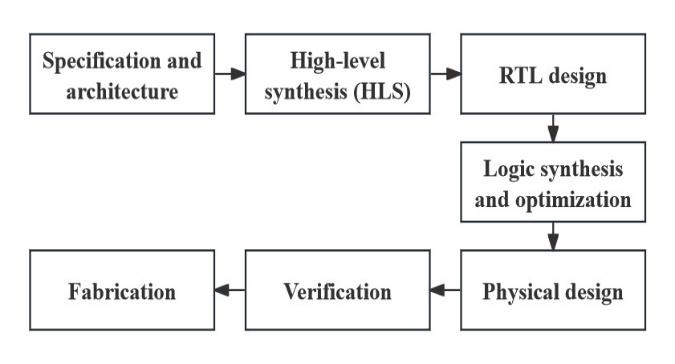
\includegraphics[width=0.8\textwidth]{images/figure-2-1-layout-EDA-flow.jpeg}
    \caption{基于强化学习的EDA流程}
    \label{fig:rl-eda-flow}
\end{figure}

\subsection{电路验证与测试}

RL在优化问题解决方面的应用可以扩展至电路的验证和测试阶段。RL通过学习验证测试的结果,优化测试策略,减少测试时间并提高测试覆盖率。\cite{1024449010.nh}

\subsection{设计知识的转移和复用}

RL算法能够将在一个设计问题中获得的知识迁移到另一个相关问题上,实现设计知识的复用。这对于处理模拟CMOS电路设计中的复杂和定制化问题尤其有价值。RL在不同设计案例中的应用,说明了其在知识迁移方面的能力。\cite{6565786}

\subsection{挑战与机遇}

总结而言,RL作为AI的一个重要分支,在模拟CMOS电路设计中的应用前景广阔。通过不断的研究和实践,RL有望在未来的模拟CMOS电路设计中发挥更大的作用,提高设计效率,优化电路性能,并推动EDA领域的技术进步。

\section{深度神经网络(DNN)在模拟CMOS电路设计优化中的应用}

在模拟CMOS电路设计的自动化进程中,深度神经网络(DNN)的进化优化算法扮演着越来越重要的角色。这些算法通过DNN的强大建模能力,预测电路设计的性能,从而减少必要的仿真次数,加速设计过程。以下是对这一主题的详细讨论,结合相关研究内容进行分析。\cite{8942062}

\subsection{优化算法在模拟电路设计中的应用}

进化优化算法,如遗传算法和粒子群优化,因其在处理复杂、多峰值问题时的有效性而被广泛应用于模拟电路设计中。这些算法通过模拟自然选择和遗传机制,迭代地从一组候选解中寻找最优解。然而,这些方法通常需要大量的仿真评估,导致计算成本和时间上的不切实际。\cite{8904889}

\subsection{深度神经网络在提高样本效率中的作用}

深度神经网络(DNN)通过其多层结构能够学习复杂的非线性关系,非常适合于预测电路设计的性能。在相关研究中,研究者提出了一个结合DNN的进化优化框架,该框架使用DNN作为判别器来预测新生成样本的性能,从而在进行实际仿真之前筛选掉不良的设计样本,显著提高了样本效率。\cite{8005220}

\subsection{BagNet框架的实现和效果}

BagNet框架的核心在于一个DNN模型,\cite{xu2020autodnnchip} 该模型被训练为能够区分生成样本的质量。这种训练方法使得DNN能够学习如何比较两个设计的性能,并预测哪个设计在每个指标上更优。BagNet框架的实验结果表明,使用该框架能够在保持设计质量的同时,显著减少仿真次数,提高了样本效率。

\subsection{实验结果和应用案例}

在设计光学链路接收器布局的案例中,BagNet框架仅使用了348次后布局仿真,相比没有使用DNN判别器的进化算法,提高了200多倍的样本效率。这一结果表明,结合DNN的进化优化算法在模拟电路设计中具有巨大的潜力。

\subsection{挑战和未来方向}

尽管结合DNN的进化优化算法显示出巨大的潜力,但仍面临一些挑战,包括DNN模型的泛化能力、对大量标注数据的依赖、以及在设计空间快速变化时模型的适应性。未来的研究可能会集中在提高DNN的泛化能力、减少对标注数据的需求、以及开发更高效的算法来处理设计空间的动态变化。\cite{9104667}

\subsection{结论}

结合深度神经网络的进化优化算法为模拟CMOS电路设计提供了一种高效的自动化设计方法。通过预测电路设计的性能,这种方法显著提高了样本效率,减少了必要的仿真次数,从而加速了设计过程。随着人工智能技术的不断进步,这种方法有望在未来的EDA工具中发挥更大的作用,推动模拟电路设计领域的发展。

\section{快速迁移设计到新工艺技术节点}

\subsection{人工智能在设计迁移中的作用}

随着集成电路技术的不断进步,模拟CMOS电路设计领域正面临着前所未有的挑战。为了保持竞争力,设计团队需要快速地将设计迁移到新的工艺技术节点,以利用更先进的制造工艺带来的性能提升和功耗降低。然而,这一过程复杂且耗时,涉及原理图的捕获或迁移、跨多个PVT(过程、电压、温度)角落的仿真和设计中心化、从头开始的布局实现,以及在后布局仿真中考虑布局寄生参数的验证。任何环节的失败都可能导致设计团队陷入漫长的迭代周期,严重影响产品上市时间。

\subsection{案例研究:从三星14nm节点迁移到5nm节点}

在三星SAFE论坛上展示的案例研究中,一个电压带隙参考(VBGR)电路从三星14nm工艺迁移到5nm工艺的过程,展示了AI在模拟设计迁移中的应用。\cite{synopsys20231102}
这个过程通常包括以下几个步骤:

\begin{enumerate}
    \item \textbf{自动化原理图迁移}:通过Custom Compiler工具,可以一键设置设备和参数在不同工艺节点之间的映射关系,实现原理图的自动迁移。
    \item \textbf{基于ML的自动布局迁移}:利用机器学习算法,可以根据原始的14nm设计自动生成符合5nm设计规则的新布局,同时保持与原始设计相似的布局结构。
    \item \textbf{基于AI的设计优化}:迁移到5nm后,使用Synopsys PrimeWave AI-based design optimization solution对设计进行跨360个PVT角落的优化,确保设计在所有条件下都能满足规格要求。
\end{enumerate}

\begin{figure}[htbp]
    \centering
    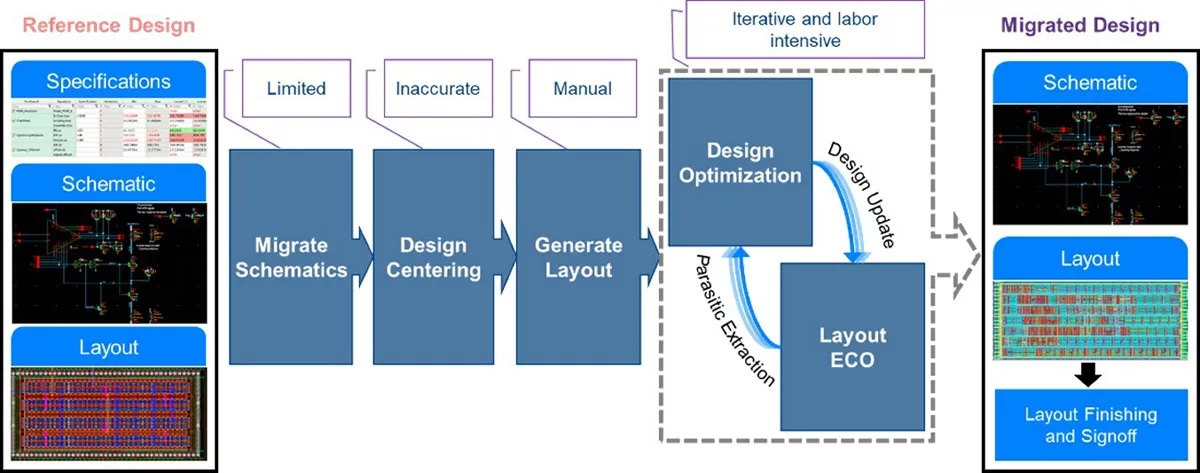
\includegraphics[width=0.8\textwidth]{images/figure-2-3-layout-migration.jpeg}
    \caption{AI驱动的设计迁移解决方案}
    \label{fig:ai-design-migration}
\end{figure}

\begin{figure}[htbp]
    \centering
    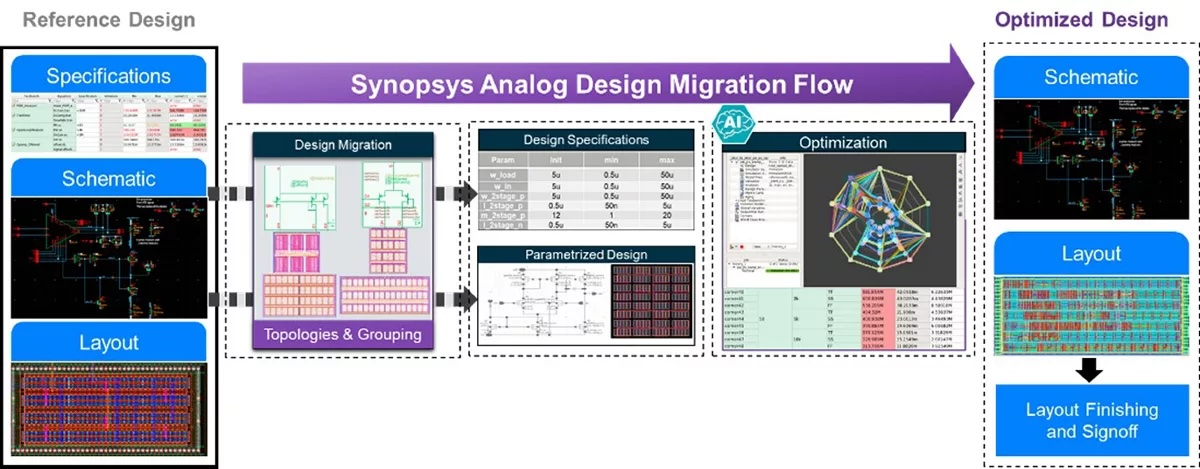
\includegraphics[width=0.8\textwidth]{images/figure-2-3-analog-design-migration-flow.jpg}
    \caption{模拟设计迁移流程}
    \label{fig:analog-design-migration-flow}
\end{figure}

\begin{figure}[htbp]
    \centering
    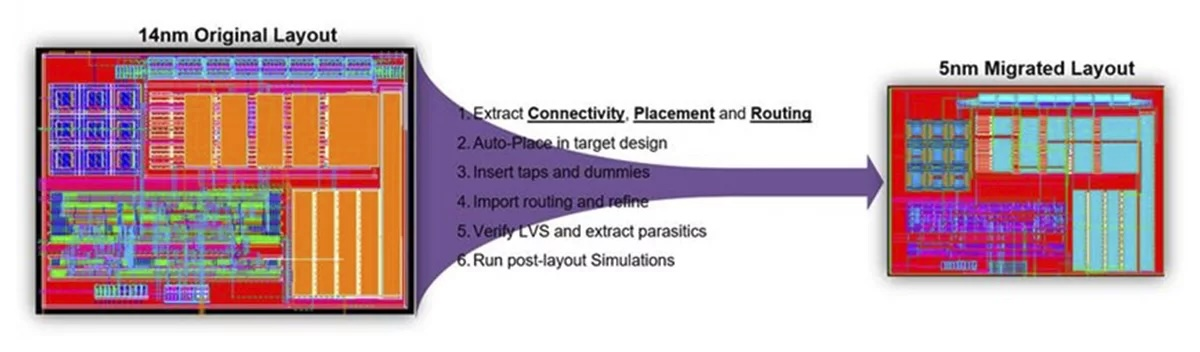
\includegraphics[width=0.8\textwidth]{images/figure-2-3-analog-migrated-layout-cd-blog.jpeg}
    \caption{迁移后的布局}
    \label{fig:analog-migrated-layout-cd-blog}
\end{figure}

\subsection{结果与影响}

通过AI驱动的设计迁移解决方案,原本需要数天才能完成的设计优化任务在几个小时内就能完成。这种快速的设计收敛不仅大大提高了设计效率,还确保了设计质量,减少了人为错误的可能性。此外,该解决方案还适用于层次结构和混合设计,包括晶体管、被动元件和其他宏块,显示出广泛的适用性。

人工智能在模拟CMOS电路设计中的应用,特别是在快速迁移设计到新工艺技术节点方面,展示了其巨大的潜力和价值。通过自动化的原理图迁移、基于ML的布局迁移和AI-based design optimization,AI技术不仅提高了设计迁移的速度和准确性,还为设计团队提供了更高效的工具,以应对日益复杂的设计挑战。随着AI技术的不断进步,预计其在模拟电路设计领域的应用将更加广泛,为集成电路设计带来革命性的变化。
